\chapter{多跳长路径上多节点联合数据认证}
本章研究设计面向规模化无线传感网的多节点联合数据认证机制。
3.1节提出了多节点联合的数据认证模型和设计目标。
3.2节设计实现了多跳长路径上多节点联合的数据认证机制。
3.3节提出了面向3.2数据认证机制的路径上节点关系维护方案。

\section{无线传感网数据认证模型}

\subsection{无线传感网中数据认证场景}
无线传感网被广泛应用在环境监测、数据采集等领域中。如图~\ref{fig:wsn}所示是一个典型的无线传感网的应用场景,
在每个监测区域中,部署的传感器节点采集数据或感知事件后将数据发送给相应的簇头节点。簇头节点将接收到的数据进行
聚合之后,通过其与基站之间的若干传感器节点传输给基站。
\begin{figure}[htbp]
  \centering
  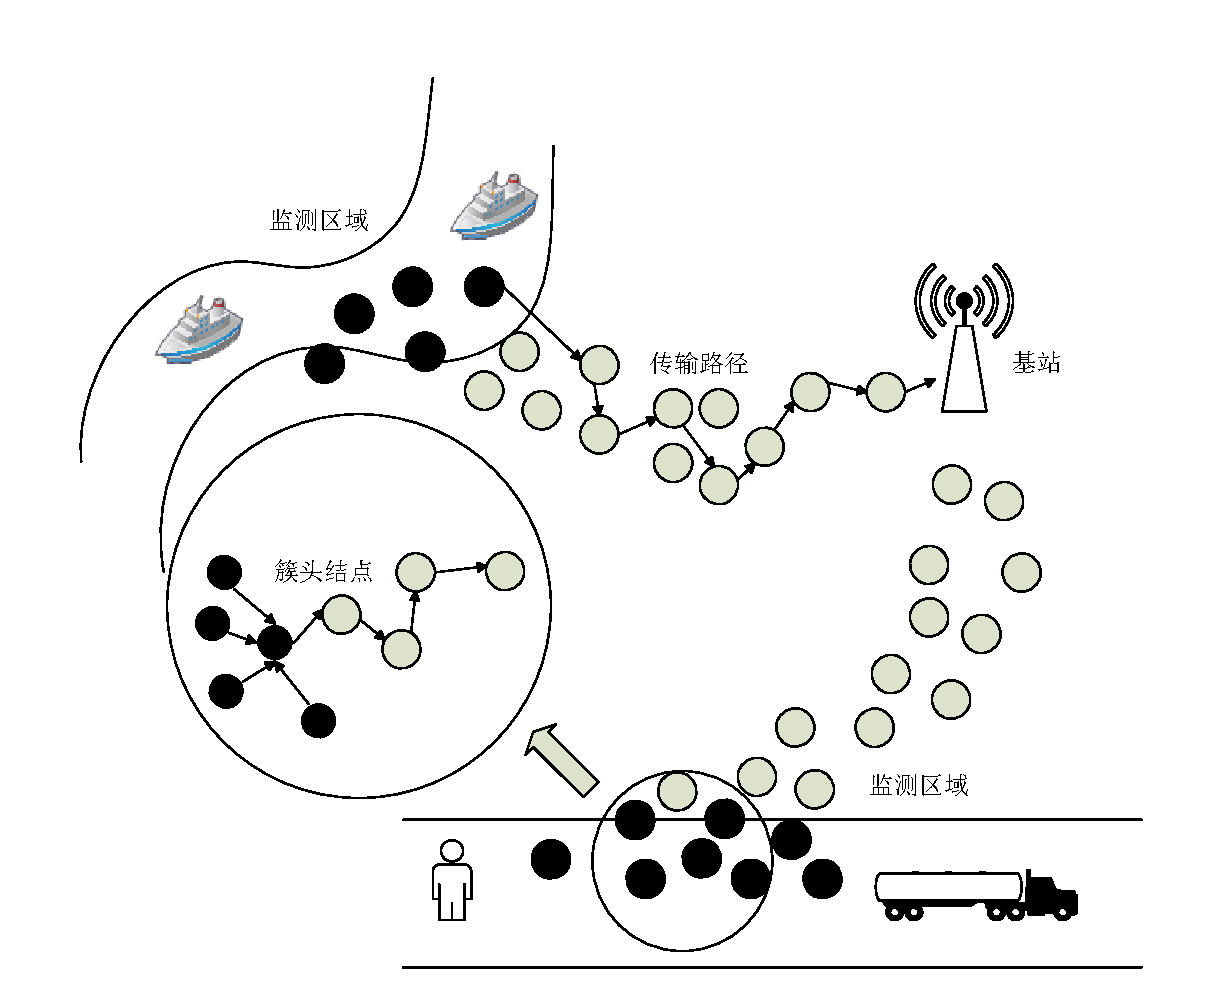
\includegraphics[width=5in]{wsnapp}
  \caption{无线传感网应用场景}
  \label{fig:wsn}
\end{figure}

无线传感网的认证包括传感器节点认证和数据认证,本文主要讨论数据认证。
传统的无线传感网认证方式是相邻节点,也即单跳之间利用预分配的密钥进行认证。由于无线传感器节点发射功率等的限制,
通信范围很小,攻击者很容易通过针对性地攻击或捕获节点,获取到密钥信息,从而攻破整个网络的认证系统。
利用预共享密钥密钥和节点信息生成节点间的共享对密钥,然后使用共享对密钥认证报文,能提高传感器网络的抗攻击的能力。

完全依靠广播传输机制,在大规模大数据无线传感网中,传输效率过低,消耗的传输能量和资源过大。有效利用大规模传感网中多跳长路径进行端对端数据传输,能够有效的保证传输效率。
%如果仅应用节点间的共享对密钥进行数据认证,路径中出现妥协节点时,整条路径的认证系统都会被攻破。
但是由于无线传感网部署环境恶劣、无人值守等原因,节点很容易被捕获或者被入侵,发送大量错误数据或垃圾数据,消耗传感器节点的能量,传统的认证机制无法对抗这种攻击。
本文研究的多节点联合数据认证机制,利用路径上多节点联合进行认证,能够有效地检测出垃圾报文,节约节点的能量。多节点联合数据认证通过维护传输路径上节点对之间的共享密钥,相隔多跳进行认证,有效提高认证系统抗攻击能力。

\subsection{多节点联合数据认证系统模型和设计目标}
\subsubsection{系统模型}
由于无线传感器节点的通信是基于广播的,所以攻击者很容易监听所有通信,注入虚假数据报文。本文假设当攻击者能够获得妥协节点的完全控制,可以获取节点中的所有密钥信息,并利用其发送虚假报文或者丢弃正常报文。攻击者的主要攻击手段是通过发送大量的虚假数据报文,达到消耗传感器节点能量的目的。
在本文的认证机制研究中假设攻击者能够有针对性地入侵节点,并利用妥协节点之间的联合来对抗认证机制。
%详述攻击模型

多节点联合数据认证的系统模型如图~\ref{fig:model}所示,主要由密钥分配、轻量MAC码和节点维护三部分组成。
\begin{figure}[htbp]
  \centering
  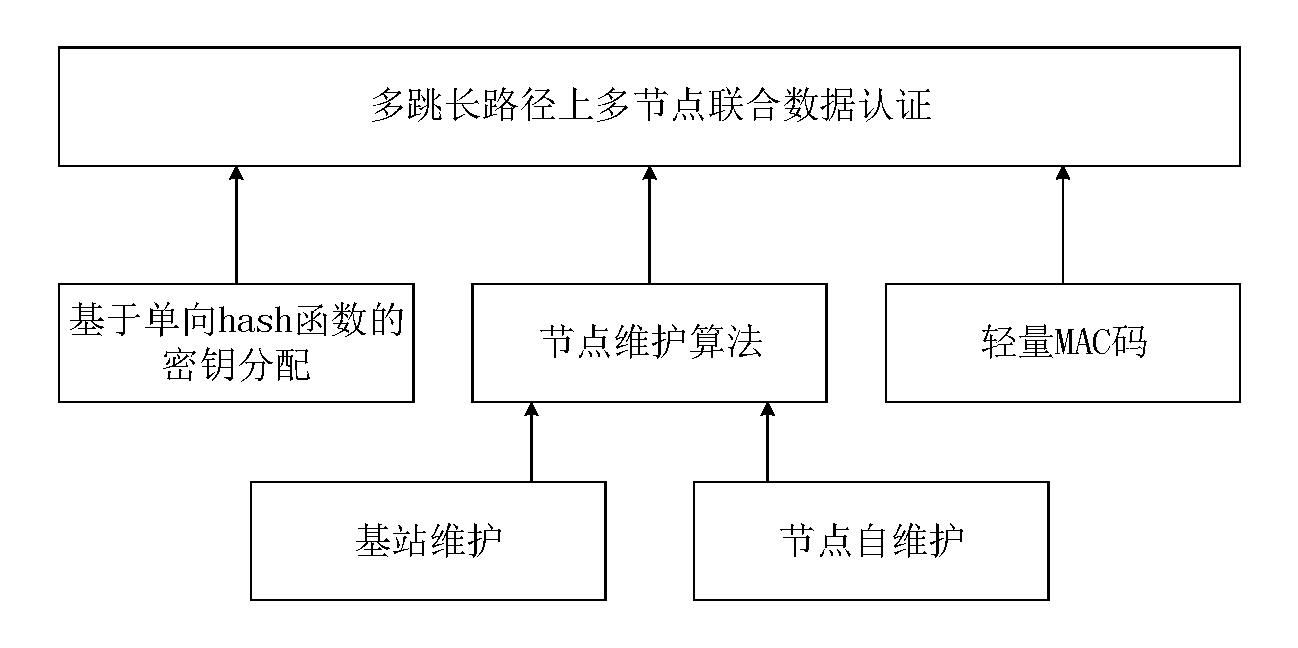
\includegraphics[width=5in]{model}
  \caption{多节点联合数据认证系统模型}
  \label{fig:model}
\end{figure}



本文中我们假设每个节点同基站之间都有共享密钥,而且每个节点都与它一跳内的相邻节点建立了对密钥,利用LEAP\upcite{c3:zhu2006leap}中提出的对密钥建立方案可以实现这个目标。
通过使用\upcite{c2:liu2005establishing,c2:du2005pairwise} 等密钥建立方案,
不相邻的节点之间可以建立对密钥,并在节点发现阶段获得对方的节点ID信息。簇与基站之间通过发现簇头之间的对密钥,形成多跳长路径,进行数据报文传输。

%添加关于簇头选举
%A Dynamic en-routing filtering scheme

\subsubsection{设计目标}
本章所研究的多跳长路径上多节点联合的数据认证机制包括如下设计目标:
\begin{enumerate}\setlength{\itemsep}{-\itemsep}
  \item 基站能够检测出所有虚假数据报文,保证传感网监测功能不受虚假报文的干扰。
  \item 当被入侵或捕获的节点数不大于t(t为系统设计参数)时,能保证虚假数据报文被丢弃。
  \item 传输路径注入的虚假数据报文,被检测并丢弃前经过尽量少的跳数,对于给定的t,我们的多节点联合认证系统有相应的虚假数据报文传播跳数上限。
  \item 认证机制计算高效,消耗能量小,适应无线传感网的要求。
  \item 能够有效应对节点失效,能够对传输路径上的节点关系进行维护,保证认证机制的稳定性。
\end{enumerate}

\section{多跳长路径上多节点联合的数据认证机制设计与实现}
\subsection{符号与定义}
本文中相关的符号定义如表~\ref{tab:notation}所示:
\begin{table}[htb]
  \centering
  \begin{minipage}[t]{0.8\linewidth} % 如果想在表格中使用脚注,minipage是个不错的办法
  \caption[相关符号说明]{相关符号说明}
  \label{tab:notation}
    \begin{tabular*}{\linewidth}{lp{10cm}}
      \toprule[1.5pt]
      {\hei 符号} & {\hei 描述} \\
      \midrule[1pt]
      $CN_i$ & 簇内节点 \\
      $t$ & 簇内节点个数,不包括簇头节点 \\
      $CH_i$ & 簇与基站之间长路径上的簇头节点\\
      $AK_{si}$ & ID为i的簇内节点与基站之间的共享密钥\\
      $AK_{uv}$ & 节点u与节点v之间的共享密钥\\
      $h_i$ & 簇头节点$CH_i$距离BS的跳数 \\
      $MAC(k,s)$   & 消息s通过密钥k生成的消息认证码\\
      \bottomrule[1.5pt]
    \end{tabular*}
  \end{minipage}
\end{table}

我们定义对于多跳长路径上的节点,当$|i-j|=t+1$时,$CH_i$和$CH_j$为相关节点。当$i-j=t+1$时,节点$CH_i$为节点$CH_j$的上行相关节点,节点$CH_j$为节点$CH_i$的下行相关节点。对于簇内节点,节点$CH_i$为节点$CN_i$的上行相关节点,节点$CN_i$为节点$CH_i$的下行相关节点。如图~\ref{fig:IHA1}所示,在$t=3$的簇与基站之间由8个簇头节点组成传输路径,其中$CN_3$为$CH_3$的下行相关节点,其中$CH_7$为$CH_3$的上行相关节点。
\begin{figure}[htbp]
  \centering
  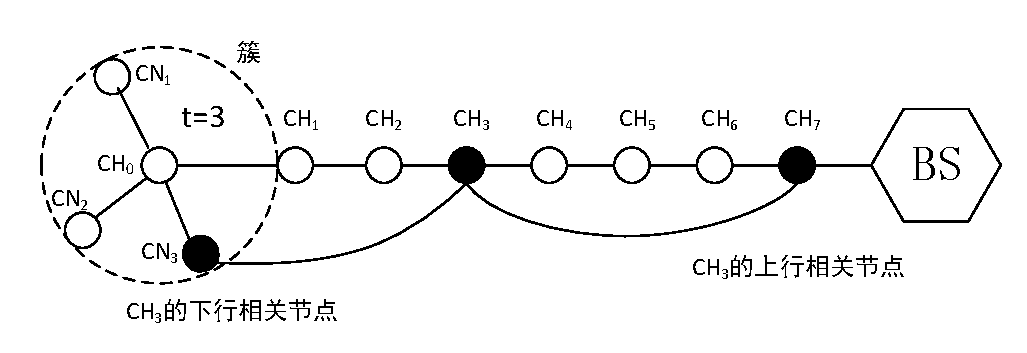
\includegraphics[width=5in]{IHA1}
  \caption{多节点联合数据认证中上下行相关节点}
  \label{fig:IHA1}
\end{figure}
\subsection{多节点联合数据认证方案}
我们的多跳长路径上多节点联合数据认证方案主要包括初始化、数据报文发送、路径中过滤、基站认证四个阶段。
\subsubsection{初始化}
传感器节点被部署到目标区域时会被分配唯一的ID和足够的密钥材料,保证每个节点与基站之间都有唯一的共享密钥$AK_{si}$。

在初始化阶段节点要获取上下行相关节点信息,在我们的多节点联合数据认证方案中,基站(Base Station,BS)会广播一个HELLO报文。簇头节点在收到HELLO 报文以后,保存$t+1$个ID信息作为上行节点,用自己的ID替换掉报文中距离自己$t+1$跳的节点的ID,其中被替换的ID信息作为其上行相关节点的ID,然后将报文继续广播。簇头节点会把该HELLO 报文中$t+1$ 个ID 分别发送给$t+1$ 个簇节点,包括簇头节点,这样每个节点都获得了上行相关节点的ID,并有了自己上行节点的ID信息。在接收HELLO报文以后每个簇头会节点记录下其到BS 之间的跳数。

簇头节点会向BS发送一个ACK报文,其中包括$t+1$个簇节点的ID。当簇节点的上行相关节点受到该ACK报文以后,保存下$t+1$个ID信息作为其下行相关节点,其中相距离自己$t+1$跳的节点的ID作为其下行相关节点ID,用自身的ID替换以后转发。BS收到ACK报文以后就建立了一条从簇到BS 的多跳长路径,而且各个节点都发现了其上下行相关节点的ID,并有了自己下行节点的ID信息。
\subsubsection{数据报文发送}
簇节点监测到事件E以后,必须要$t+1$个节点都发出报文才能确认监测到的事件,如果没有至少$t+1$个节点的报文,则认为是无效事件。

簇节点$CN_i(1\leq i\leq t)$对于事件E首先使用其与BS之间的共享密钥$AK_{si}$计算消息认证码$MAC(AK_{si},E)$,称其为簇节点MAC,并使用其与上行相关节点$CH_i$的共享密钥计算消息认证码$MAC(AK_{CN_i CH_i},E)$,称其为相关节点MAC。簇头节点$CH_0$ 从$t+1$个簇节点(包括簇头节点)收集到$t+1$份报文后对数据进行整合后发送。如图~\ref{fig:IHA2}所示,是一个事件E被感知和发送的过程。
\begin{figure}[htbp]
  \centering
  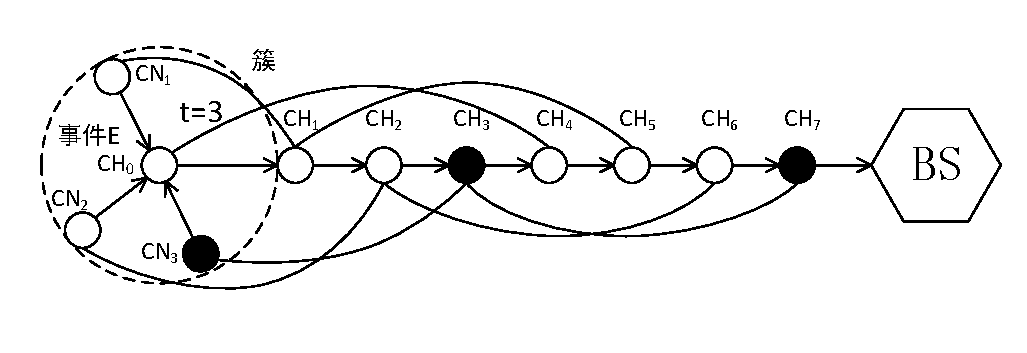
\includegraphics[width=5in]{IHA2}
  \caption{多节点联合数据认证中数据报文发送过程}
  \label{fig:IHA2}
\end{figure}

在图~\ref{fig:IHA2}的传输过程中,簇头节点$CH_0$收到簇节点的数据报文以后,对每个节点的簇节点MAC使用XOR运算进行压缩,缩小传输报文的大小,降低节点能量消耗,记作$XMAC(E)$:
\begin{equation}\label{XMAC}
\begin{split}
  XMAC(E)
  &=MAC(AK_{s1},E)\oplus MAC(AK_{s2},E)\oplus MAC(AK_{s3},E)\oplus MAC(AK_{s0},E)
\end{split}
\end{equation}
簇的ID记作$C_i$,簇头节点$CH_0$距离BS的跳数记作$h$,则对于事件E簇头节点$CH_0$发给BS的报文R可以记作:
\begin{equation}\label{report}
\begin{split}
  R=
  & E,h_0,\{CH_0,CN_1,CN_2,CN_3\},XMAC(E),\{MAC(AK_{CN_1 CH_1},E),\\
  & MAC(AK_{CN_2 CH_2},E),MAC(AK_{CN_3 CH_3},E),MAC(AK_{CH_0 CH_4},E)\}
\end{split}
\end{equation}
报文R中包含了簇节点的ID:$CH_0,CN_1,CN_2,CN_3$,从而BS能够认证压缩的$XMAC(E)$。

\subsubsection{路径中过滤}
当节点$CH_i$从下行节点收到报文R以后,首先用相邻节点共享密钥对进行认证。然后使用其上下行相关节点的共享密钥对E计算MAC,并更新报文R。对于图~\ref{fig:IHA2}中的节点$CH_1$,收到来自$CH_0$的报文后,使用与其下行相关节点$CN_1$之间的共享密钥对E 计算消息认证码$MAC(AK_{CH_1 CN_1},E)$,与报文R中的第$(h_0 - h_i)-((h_0 - h_i)/(t+1))\ast (t+1)=1$个相关节点MAC,$MAC(AK_{CN_1 CH_1},E)$ 进行比较,如果不同则丢弃报文R;如果相同,使用与其上行相关节点$CH_5$之间的共享密钥对E计算消息认证码$MAC(AK_{CH_1 CH_5},E)$,并替代原报文R中的$MAC(AK_{CN_1 CH_1},E)$,并将其转发给下一节点,更新后发送给节点$CH_2$的报文R为:
\begin{equation}\label{report}
\begin{split}
  R=
  & E,C_i,h_0,\{CH_0,CN_1,CN_2,CN_3\},XMAC(E),\{MAC(AK_{CN_1 CH_5},E),\\
  & MAC(AK_{CN_2 CH_2},E),MAC(AK_{CN_3 CH_3},E),MAC(AK_{CH_0 CH_4},E)\}
\end{split}
\end{equation}
\subsubsection{基站认证}
当BS收到报文R后,使用BS与报文R节点ID列表中$t+1$个簇节点之间的共享密钥计算MAC,并用XOR运算计算这$t+1$个MAC的值,与报文R中的XMAC比较,如果不同,则丢弃报文。如果相同,则对事件E作出响应。
\subsection{安全性能分析}
由于我们的方案使用了XOR运算压缩的XMAC保证了BS能检测出所有的错误报文,并且有相邻节点认证,下面我们对多节点联合认证的安全性能进行分析时,仅讨论路径中过滤的情况。

当一个节点被捕获时,攻击者就能获得一个能经过认证的MAC来欺骗它的上行相关节点。当传感器传输路径中被捕获的节点达到$t$个时,则攻击者可以用$t$个MAC组成的报文欺骗$t$个未被攻击的上行相关节点。但是我们的多节点联合数据认证机制需要$t+1$个有效MAC 才能通过认证,攻击者的入侵报文会被某个未被攻击的节点丢弃,因为它下行相关节点的MAC是无效的。因此我们的方案能保证当攻击者没有捕获超过$t$个节点的时候,入侵报文在被丢弃前仅能欺骗$t$个未被攻击节点。

通过上面的分析,我们的多节点联合数据认证机制的安全性是基于上下行相关节点间的认证的。我们下面对攻击者捕获了最多$t$个节点情况下的安全性进行分析,路径中过滤的攻击主要包括两个部分,簇内节点攻击和路径中节点攻击。
\subsubsection{簇内节点攻击}
当所有被攻击的$t$个节点都是簇内节点,没有路径中的节点被捕获时,不管簇头节点有没有被捕获,数据报文R中的$t+1$个MAC中总会有一个是无效MAC,从而被离簇头最近的$t+1$个路径节点(如图~\ref{fig:IHA2}中的节点$CH_1,CH_2,CH_3,CH_4$)中的某个检测出来并丢弃。
说明簇内节点攻击中,错误数据报文仅能欺骗最多$t$个未被攻击节点。

\subsubsection{路径中节点攻击}
我们讨论被攻击的$t$个节点在初始化阶段的ACK过程中能协作进行攻击的情况。我们讨论最坏情况,当被捕获的$t$个节点中包括了簇头节点$CH_0$,且从$CH_0$到BS之间间隔$t$个未被捕获节点均匀分布,可以表示为:
\begin{equation}
\begin{split}
  & CH_0,\{CH_{1,1},CH_{1,2},\cdots,CH_{1,t}\},N_1,\{CH_{2,1},CH_{2,2},\cdots,CH_{2,t}\},\\
  & N_2,\cdots,N_{t-1},\{CH_{t,1},CH_{t,2},\cdots,CH_{t,t}\},\cdots,BS
\end{split}
\end{equation}
其中$CH_0,N_1,N_2,\cdots,N_{t-1}$是被捕获的$t$个节点,任意两个被捕获节点被$t$个未被捕获节点分隔。

在初始化阶段,簇头节点$CH_0$在ACK阶段通过发送一个伪造的ID信息组,$y,CH_0,N_1,N_2,\cdots,N_t$,其中$y$为任意伪造的节点信息,使得上下行相关关系确定过程中,未被捕获节点的下行相关节点都为被捕获节点。由于间隔$t$个未被捕获节点之后,是一个被捕获的节点$N_i$,伪造的ACK 不会因为$y$是伪造的节点信息而被丢弃,而是重新将$y,CH_0,N_1,N_2,\cdots,N_t$转发给上行节点。完成了ACK过程以后,所有的未被捕获节点的下行相关节点都是被捕获节点。

簇头节点$CH_0$发送的错误数据报文R可以表示为:
\begin{equation}\label{report}
\begin{split}
  R=
  & E,C_i,h_0,\{CH_0,CN_1,\cdots,CN_t\},XMAC(E),\{MAC(AK_{N_t CH_1},E),\\
  & MAC(AK_{N_{t-1} CH_2},E),\cdots,MAC(AK_{CH_0 CH_t},E),MAC(AK_y,E)\}
\end{split}
\end{equation}
其中$MAC(AK_y,E)$为伪造的MAC。这个错误的数据报文能欺骗$t^2$个未被捕获节点,也就是攻击者捕获了最多$t$个节点时最坏的情况。
\section{路径上节点关系的维护方案}
我们的多节点联合数据认证机制是基于节点的上下行相关关系的,每个节点需要在初始化阶段发现其上行相关节点ID和下行相关节点ID,这样才能通过节点间的共享对密钥计算MAC,对数据报文进行认证。如果基站和簇头节点之间的多跳长路径是静态的,那只需要在初始化阶段进行一次上下行相关节点发现。但是由于无线传感网的特性,簇头节点在簇内是选举产生的,经常发生变化,还有传感器节点由于环境原因或者遭受攻击都有可能失效,导致路径的变化。因而需要对路径节点的上下行相关关系进行维护,以适应无线传感网的变化。下面从基站维护和节点自动维护两个情况介绍节点关系的维护。
%在拓扑结构变化不大的基础上。
\subsection{基站维护}
在相对稳定的无线传感网传输路径上,BS会周期性广播信标消息,信标信息中捎带每个节点的ID信息。
在初始化阶段,每个簇头节点都记录了自己到BS之间的跳数$h$。当一个节点收到信标消息以后,如果$h\geq t+1$,则检查该消息中$t+1$个上行节点的ID,如果$h< t+1$,则检查该消息中$h$个上行节点的ID。如果所有上行节点ID信息没有变化,路径中该节点的上行节点没有变化。如果有变化则在发送给BS的信标消息中附带节点变化消息,BS重新发送HELLO报文,进行上下行相关节点发现的过程。
\subsection{节点自动维护}
在基站维护的过程中,如果信标消息的广播周期较短,会造成大量的数据传输,消耗传感器节点的能量;如果信标消息的广播周期较长,那么部分节点失效或被攻击就会造成大量的数据报文被丢弃,所以我们需要节点自动维护的机制,修复路径中的节点上下行相关关系。
\begin{figure}[htbp]
  \centering
  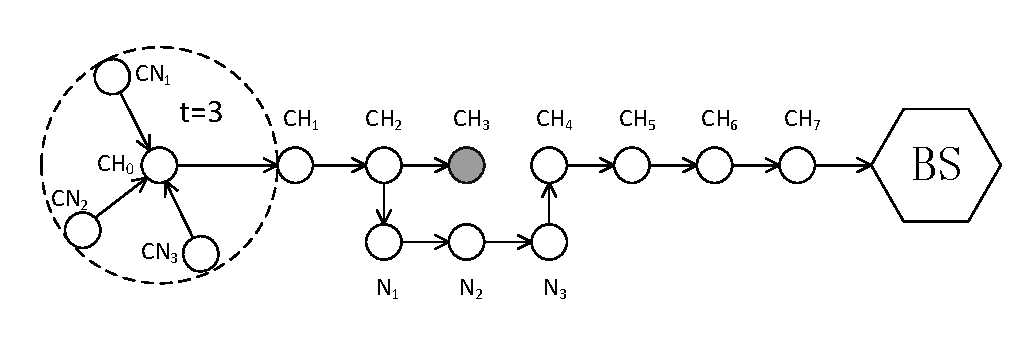
\includegraphics[width=5in]{IHA3}
  \caption{节点自动维护上下行相关关系的过程}
  \label{fig:IHA3}
\end{figure}

我们的节点自动维护机制是基于GPSR协议\upcite{c3:karp2000gpsr}中的右手准则的。我们假设每个节点都自动相邻节点的相对位置。如图~\ref{fig:IHA3}所示是一个节点自动维护的过程,当节点$CH_2$检测到$CH_3$失效以后,给它的逆时针方向的第一个相邻节点$N_1$ 发送一个修复消息,消息中包括了$CH_2$的$t$个上行节点的ID,$\{CH_4,CH_5,CH_6\}$,不包括$CH_3$。$N_1$,$N_2$按照初始化阶段的规则进行转发,当$N_3$收到修复消息以后,发现消息中有$CH_4$的ID,是它的相邻节点,这样就发现了一条替代路径。$N_3$将消息发送给$CH_4$以后,$CH_4$将上行节点ID,$\{CH_4,CH_5,CH_6,CH_7\}$捎带在消息中转发给$N_3$,同初始化阶段的HELLO报文。完成这些过程以后,新路径上的节点就建立上下行相关关系,也就是修复了这条长路径。

\section{本章小结}
本章提出了无线传感网中数据认证模型,针对相关攻击模型,提出了多跳长路径上多节点联合的数据认证方案。设计实现了多节点联合数据认证协议,并对其安全性能进行了分析。为了维持多节点联合数据认证机制的稳定性,设计了路径上相关节点关系维护的机制。


